\documentclass[11pt,]{article}
\usepackage[left=1in,top=1in,right=1in,bottom=1in]{geometry}
\newcommand*{\authorfont}{\fontfamily{phv}\selectfont}
\usepackage[]{mathpazo}


  \usepackage[T1]{fontenc}
  \usepackage[utf8]{inputenc}



\usepackage{abstract}
\renewcommand{\abstractname}{}    % clear the title
\renewcommand{\absnamepos}{empty} % originally center

\renewenvironment{abstract}
 {{%
    \setlength{\leftmargin}{0mm}
    \setlength{\rightmargin}{\leftmargin}%
  }%
  \relax}
 {\endlist}

\makeatletter
\def\@maketitle{%
  \newpage
%  \null
%  \vskip 2em%
%  \begin{center}%
  \let \footnote \thanks
    {\fontsize{18}{20}\selectfont\raggedright  \setlength{\parindent}{0pt} \@title \par}%
}
%\fi
\makeatother




\setcounter{secnumdepth}{3}

\usepackage{longtable,booktabs}

\usepackage{graphicx,grffile}
\makeatletter
\def\maxwidth{\ifdim\Gin@nat@width>\linewidth\linewidth\else\Gin@nat@width\fi}
\def\maxheight{\ifdim\Gin@nat@height>\textheight\textheight\else\Gin@nat@height\fi}
\makeatother
% Scale images if necessary, so that they will not overflow the page
% margins by default, and it is still possible to overwrite the defaults
% using explicit options in \includegraphics[width, height, ...]{}
\setkeys{Gin}{width=\maxwidth,height=\maxheight,keepaspectratio}

\title{Estudio Profundizado y comparativo de la cuenca del Soco\\
Subtítulo\\
Subtítulo  }



\author{\Large Isaac De La Rosa\vspace{0.05in} \newline\normalsize\emph{Estudiante de la Licenciatura en Geografia Mencion Representacion
Espacial en la Universida Autonoma de Santo Domingo (UASD)}  }


\date{}

\usepackage{titlesec}

\titleformat*{\section}{\normalsize\bfseries}
\titleformat*{\subsection}{\normalsize\itshape}
\titleformat*{\subsubsection}{\normalsize\itshape}
\titleformat*{\paragraph}{\normalsize\itshape}
\titleformat*{\subparagraph}{\normalsize\itshape}

\titlespacing{\section}
{0pt}{36pt}{0pt}
\titlespacing{\subsection}
{0pt}{36pt}{0pt}
\titlespacing{\subsubsection}
{0pt}{36pt}{0pt}





\newtheorem{hypothesis}{Hypothesis}
\usepackage{setspace}

\makeatletter
\@ifpackageloaded{hyperref}{}{%
\ifxetex
  \PassOptionsToPackage{hyphens}{url}\usepackage[setpagesize=false, % page size defined by xetex
              unicode=false, % unicode breaks when used with xetex
              xetex]{hyperref}
\else
  \PassOptionsToPackage{hyphens}{url}\usepackage[unicode=true]{hyperref}
\fi
}

\@ifpackageloaded{color}{
    \PassOptionsToPackage{usenames,dvipsnames}{color}
}{%
    \usepackage[usenames,dvipsnames]{color}
}
\makeatother
\hypersetup{breaklinks=true,
            bookmarks=true,
            pdfauthor={Isaac De La Rosa (Estudiante de la Licenciatura en Geografia Mencion Representacion
Espacial en la Universida Autonoma de Santo Domingo (UASD))},
             pdfkeywords = {Geomorfología fluvial, Morfometría de Cuenca, Analisis Morfométrico},  
            pdftitle={Estudio Profundizado y comparativo de la cuenca del Soco\\
Subtítulo\\
Subtítulo},
            colorlinks=true,
            citecolor=blue,
            urlcolor=blue,
            linkcolor=magenta,
            pdfborder={0 0 0}}
\urlstyle{same}  % don't use monospace font for urls

% set default figure placement to htbp
\makeatletter
\def\fps@figure{htbp}
\makeatother

\usepackage{pdflscape} \newcommand{\blandscape}{\begin{landscape}}
\newcommand{\elandscape}{\end{landscape}} \usepackage{float}
\floatplacement{figure}{H}
\newcommand{\beginsupplement}{ \setcounter{table}{0} \renewcommand{\thetable}{S\arabic{table}} \setcounter{figure}{0} \renewcommand{\thefigure}{S\arabic{figure}} }


% add tightlist ----------
\providecommand{\tightlist}{%
\setlength{\itemsep}{0pt}\setlength{\parskip}{0pt}}

\begin{document}
	
% \pagenumbering{arabic}% resets `page` counter to 1 
%
% \maketitle

{% \usefont{T1}{pnc}{m}{n}
\setlength{\parindent}{0pt}
\thispagestyle{plain}
{\fontsize{18}{20}\selectfont\raggedright 
\maketitle  % title \par  

}

{
   \vskip 13.5pt\relax \normalsize\fontsize{11}{12} 
\textbf{\authorfont Isaac De La Rosa} \hskip 15pt \emph{\small Estudiante de la Licenciatura en Geografia Mencion Representacion
Espacial en la Universida Autonoma de Santo Domingo (UASD)}   

}

}








\begin{abstract}

    \hbox{\vrule height .2pt width 39.14pc}

    \vskip 8.5pt % \small 

\noindent Como una ciencia complementaria de la geografía física, la geomorfología
ha sido una de las mas importantes al momento de crear una perspectiva
real del relieve, siendo este util para explicar causas y consecuencias
de movimientos y poder describir los mismos. Dentro de este encontramos
la geomorfología fluvial, que como etimológicamnte se indica, es la
encargada de describir los procesos fluviales en la litosfera, asi como
tambien sus causas y consecuencias en su paso por la corteza terrestre,
Pero notese lo poco atendido que está la morfometría fluvial en nuestro
pais. Muchas fuentes afirman que el funcionamiento de una cuenca se
asemeja al de un colector que recibe la precipitación y la convierte en
escurrimiento superficial o sub superficial; esta transformación depende
de las condiciones climáticas y las características físicas de la
cuenca. La República Dominicana nunca ha tenido como fin el desarrollo
de cualquier ciencia geográfica para la obtencion de informacion crucial
de la realidad geográfica puesto que la morfometría fluvial explica con
mejor perspectiva las razones hidrológicas, esta tambien describe su
organizacion fluvial, ordenes de red, drenajes, puntos mas elevados,
cursos mas cortos y mas largos. El análisis realizado a La cuenca del
Soco arroja resultados impresionantes, cuales explican que tiene como
área unos 988.62 km2 y un perimetro de 227.63 km, siendo esta la cuenca
mas grande de la region este, esta logra una elevacion maxima de
646.96m, la elevacion media 136.34m y la elevación mínima 0.032. Dicha
cuenca localizada en la región este del país, iniciando entre las
subregiones Yuma y Higüamo, con desembocadura en la boca del soco. Se
comprueba en los perfiles longitudinales los cursos concavos y los
cursos convexos. se comprueba que la curva e integral hipsométrica está
asociada a factores evolutivos de las regiones que posee el relieve.
Este Análisis asi como muchos otros ponen en veracidad lo eficáz que
puede llegar a ser la tecnología geoespacial para el análisis
cuantitativo basado en una cuenca hidrografica, sin importar su tamaño.


\vskip 8.5pt \noindent \emph{Keywords}: Geomorfología fluvial, Morfometría de Cuenca, Analisis Morfométrico \par

    \hbox{\vrule height .2pt width 39.14pc}



\end{abstract}


\vskip 6.5pt


\noindent  \section{Introducción}\label{introducciuxf3n}

Nunca ha sido tan importante como hoy conocer Las características
físicas de una cuenca de drenaje, las cuales revisten gran importancia
para la realización de estudios geomorfológicos, hidrológicos y
geotécnicos, ya que influyen en el desarrollo de múltiples procesos
fluviales y en el riesgo de inundación morfometria de cuenca. Si bien es
cierto que cada vez que se hace un estudio de este tipo o relacionado a
este, es en cierto sentido intermiable por la poca informacion ofrecida
por las partes encargadas. (Busnelli \& Horta, 2014), aunque en este
articulo tendremos la exepcion.

En la republica Dominicana, existe una cuenta, una de las mas
importantes en el este de dicho pais, el cual comprende desde la parte
norte de la region este hasta el sur de dicha region, politicamente
comenzando desde la Provincia de El Seibo y la Provincia de Hato Mayor
del rey, en las zonas muy forestales y altas de la Cordillera del Seibo
(coordillera oriental), y dicha cuenca sera el punto de concentracion de
nuestra investigacion. Posee una forma en cierto sentido pensando el
punto de desemboque, pero, ¿Posee algo mas que no sepamos? ¿que hace
esta cuenca una de las mas importantes de la region?, ¿Existe o podria
existir un area de estudio profundizado geomorfologicamente que impacto
a la sociedad geografica latinoamericana o e mundo?.

Reivindicar la geomorfología, es decir, los procesos y formas abióticos,
como valor en sí mismo del sistema fluvial y como clave de conservación
y restauración constituye una innovación en nuestro país, donde el
desconocimiento geomorfológico en el ámbito ambiental es muy grave,
donde muchas veces la geomorfología no se considera (como ocurre en
muchos estudios de impacto) y no es que se infravalore, sino que
directamente no existe o se desprecia. (Ollero et al., 2011).

El conocimiento morfometrico de las cuentas de la Republica Dominicana
es mucho menos del 30 por cierto de su totalidad, haciendo meramente
imposible los hallazgos de geogormas interesantes para estudiar y
analizar morfometricamnete profundo. sin embargo, El concepto de
Horton-Strahler ha sido importante en la geomorfología de las cuencas
fluviales; describe propiedades de escala e identifica GIUH, pero
también ha atraído críticas, porque depende del área de umbral S, que se
utiliza para extraer la red de canales de los modelos digitales de
elevación (MDE), de la posición de la salida y del escaso número de
ratios utilizados para identificar las leyes de escala. Para superar
estas limitaciones, este artículo propone nuevos índices independientes
de S y que tienen propiedades similares a las relaciones de
Horton-Strahler.(Moussa, 2009).

La Geomorfología Regional, definida como ciencia que se ocupa de
describir y explicar la distribución espacial de las formas del terreno
a escala regional y sub-regional, ha sido considerada por la
planificación física y la ordenación del territorio más clásicas, como
la única disciplina capaz de analizar las ``líneas maestras'' que
definen el carácter complejo del territorio y del paisaje.

La utilización del relieve como base física para la delimitación y
definición de unidades territoriales integradas, básicas para gestionar
el territorio y sus recursos, ha constituido además uno de los métodos
tradicionalmente empleados por algunas de las disciplinas ambientales
que en mayor medida han contribuido al acercamiento de la planificación
física clásica hacia la nueva ordenación integral; es el caso de la
Ecología del Paisaje, la Ecología Humana y la Geografía
Ambiental.(Muñoz-Rojas, Carrasco González, \& Pedraza Gilsanz, 2009).

Este trabajo muestra informacion actualizada sobre la cuenca del Soco,
centrandose su morfometria tantos aspectos sean conocidos, realizado con
apoyo de softwares libres y scripts adaptados al area de estudio, la
cuenca del Soco. También, se inquiere sobre la existencia de una
relación entre: los perfiles longitudinales e índice de concavidad con
la litología de la cuenca; la relación entre los parámetros
morfométricos con las características litológica y si hay factores que
se asocien con la curva e integral hipsométricas de la cuenca. Por medio
de parámetros morfométricos se busca identificar qué forma tienen la
cuenca y su red de drenaje. De igual manera, se trata de comprender como
se organiza la red de drenaje; y, tras el estudio de la cuenca y su red
de drenaje, se indaga si se producen ciertros movimientos de
reorganización en ellas.

\ldots

\section{Metodología}\label{metodologuxeda}

Para la realizacion de estas operaciones utilizo operaciones de analisis
morfometrico de redes de drenaje y cuenca de los paquetes de software de
codigo abierto GRASS GIS, utilizando como medio de interpretacion y
organizacion cuantitavia y/o cualitativa de informacion R como entorno
de programacion (Citeseer, n.d.). Dentro de Grass Gis fueron utilizados
otros paquetes para la optima comprension de datos, con la utilizacion
de un modelo digital de elevacion (para lo siguiente, MDE) de la mision
radar del transbordador espacia Shuttle (Lemos, Souza, \& Rocha, 2004),
con altura aproximada a 90 metros para la extraccion de informacion
requiriente.

En la acumulacion de flujo, los parametros de cuenca del mismo, demas
como elevación, drenaje, y otros mas, fueron calculados a través del
addon de GRASS GIS r.watershed (Lozar, n.d.), contando con un umbral
acumulado de 82 celdas, en un MDE. Las capas generadas se ingresaron a R
al junto de la libreria ap y al igual manejo con la libreria raster.

Para extraer la cuenca se utilizó el addon r.water.outlet (Lozar, n.d.),
usado tambien el addon r.vect, lo que llevó a convertir el raster
resultante en vectorial, para así colocacarlo en R. de igual forma se
aplicó el addon r.stream.extract (Jasiewicz, n.d.), para lograr extraer
la red de drenaje donde se llevaron a R los resultados del mismo.

Por consiguiente, en la orden de red y el analisis hortoniano, se puso
en uso el addon r.stream.extract para producir un mapa de direccion de
flujo. Por otra parte, para la creación de mapas de ordenes de red se
uso el addom r.stream.order (Jasiewicz, n.d.), en el cual se usó la
clasificacion de de Strahler para el analiside red de dicha cuenca.

Se utilizaron de igual forma los addons r.info para extraer los valores
máximos y mínimos del orden de red segun Strahler partiendo de un
raster, delimitada la cuenca a traves de la red de drenaje con
r.stream.basins (Jasiewicz, n.d.). Para el uso de estadostocas segun
orden de red de Hortonm para las redes de Strahler y Horton, se utilizó
el addon r.stream.stats (Jasiewicz, n.d.) en resumen de las
estadisticas. Para el cálculo de los índices de concavidad y los
perfiles longitudinales, en primer lugar, se extajeron los cursos mas
largos de la cuenca en cuestión a traves de la función LfpNetwork, para
luego emplear la función LfpProfilesConcavity, dicha función arrojó los
índices de concavidad para los cursos mas largos, y así mismo, sus
perfiles longitudinales.

Luego de la creación de una nueva region de GRASS en R, se llevaron a
números enteros la extensión y la resolución del DEM con las funciones
integerextent y xyvector (José Ramón Martínez Batlle, 2018). Tambien se
llegó a utilizar la herramienta gdalwarp (``GDAL-biblioteca de
abstracción de datos geoespaciales,'' n.d.) para extraer la sesion de
GRASS. se usó el addon r.stream.extract, para generar la red de drenaje
y obtener las coordenadas que mas adelante seria convetrtidas a
EPGS:4326 (Jain, n.d.), como numeros enteros con la funcion my\_trans.
(José Ramón Martínez Batlle, 2020) Mientras que, para la obtención de
los parámetros morfométricos de la cuenca se utilizó el addon r.basin
(``Un enfoque de código abierto para la caracterización fisiográfica de
la cuenca,'' n.d.). Los vectores obtenidos son transformados a EPGS:4326
(Jain, n.d.) y así siendo vistos o visualizados con la liobreria
leaflet. De igual forma, para explorar los parámetros de la cuenca fue
utuilizada la libreria readr. Para el cálculo de la curva y la integral
hipsometrica de la cuenca, en primer lugar, lo realizado fue representar
las cuencas con las librerias sp y mapview; y en segundo lugar, calcular
la integral y cuva hipsométrica mediante el uso de la función
HypsoIntCurve (José Ramón Martínez Batlle, 2018).

\ldots

\section{Resultados}\label{resultados}

En dicho estudio realizado a la cuenca del Soco utilizando el Script
Reproducible, revela información que facilita el análisis y comprensión
de la cuenca, vierase de manera agrupada como de forma desagregada. Por
consiguiente, se presentan de manera resumida, las caracteristicas
morfométricas principales de la cuenca en cuestion y su red de drenaje.

La cuenca del Soco tiene como area unos 988.62 km2 y un perimetro de
227.63 km, siendo esta la cuenca mas grande de la region este, esta
logra alcanzar una elevacion maxima de 646.96m, la elevacion media
siendo de 136.34m y la elevacion minima de 0.032, con uno de los
relieves mas heterogeneos e irregulares antes analizados. CITA DE TABLAS
2 Y 9.

Observandose la figura (\ref{mapauno}) la forma de la cuenca es
ciertamente triangular, con la parte mas ancha en el norte y la punta de
la figura en el sur con su desembocadura. Así mismo, los párametros de
coeficiente de compacidad, forma de la cuenca y razón de elongación, nos
dan la confirmación de la forma triangular de la cuenca en cuestión (ver
tabla \ref{tablanueve}). Mientras que la red de drenaje de la cuenca se
pueden ver drenajes acumulados y de cierta forma informales, siendo
densa en ramificaciones muy regulares tal vemos en la cuenca media alta,
al sur (ver figura \ref{mapanueve}); debido a que relive se denota
accidentado y a que la composición del material encontrado en la sierra
del seibo, elevaciones territoriales importantes en la región y donde
nace, por consiguiente, la cuenca del Soco.

La red de drenaje de la cuenca, Según Srahler, presenta un total de 461
redes (ver tabla \ref{tablauno}), y se organiza por ordenes desde el
numero 1 hasta la numero 5 CITAR DOS FIGURAS 6 Y 10. Donde éstas redes
de drenaje de orden uno hasta orden cinco organizados de forma
concatenada, van dando como afluentes sus aguas a un curso fluvial mayor
hasta llegar al curso principal; las de orden dos, que suman un total de
75, se ve una reduccion en el numero de redes, presentando cierto
aumento en el area del orden y descenso en las redes de drenaje de
redes, de orden 3 se encontraron 16m de orden 4 se pudo encontrar 5 y
por consiguiente, en el orden 5 solo se encontró uno solo.

En un análisis se prevee que contenga captura fluvial en los cursos mas
largos de drenaje, los cuales generaron los perfiles longitudinales y se
obtuvieron los índices de concavidad, la gran mayoría mostraron ser
positivos a la concavidad, otros salieron negativos a ella, tratandose
de unos 6 con este caso.(ver figura \ref{mapaocho}).

Los parametros morfometricos que se obtuvieron(ver tabla
\ref{tablasiete}) incluyendo coeficiente de compacidad que indica que la
forma de la superficia de la cuenca de acuerdo con su delimitacion y el
predominio en su escorrentía, es muy alargada; pero tomando en cuenta el
parametro forma de la cuenca genera un indice el cual indica que la
cuenca, ademas de ser muy alargada, es bastante ensanchada por las areas
de cuenca media y cuenca alta.

De los cursos mas largos, se destaca el numero 5 (ver figura
\ref{mapados}), siendo este meramente el rio cabecera, el rio soco, el
cual desemboca en la boca del soco al sur de la cuenca, el curso se
mueve englobado de norte a sur, presentando lineas concavas que
facilitan su curso, creando meandros en su recorrido, politicamente pasa
por 3 provincias, cauce formado por piedra caliza y conglomerados, sin
presencia de clinoformas, mientras que presenta anchura en su lecho en
la parte baja de la cuenca.

Por otra parte, en los perfiles podemos apreciar varias lineas convexas,
contando con 18 redes convexas, de ordenes menores, llamense 2,3,4, en
la parte norte de la cuenca y a los alfuentes de los alrededores, la
mayoria desde el numero 31 en adelante. La razon de bifurcacion mostrada
en los resultado de la ejecucion (ver tabla \ref{tablasiete}), muestrean
una constancia en los numeros y en el area como tal.

Tambien están los cursos casi rectilineos como son los caso del los
cursos numero 24, 37 y 47 con incides de concavidad menores a 0.18,
rectilinios a mas de 50\%. la cuencas del soco tiene 461 rios de ordenes
contables, lo que la convierte en una de las cuencas mas grandes e
importantes de ls nacion.(ver tabla \ref{tablauno})

Las estadisticas que son generadas sobre la curva y la integral
hipsometrica obtuvieron 75 resultados para los cursos que en red de
orden 2 todos con gran similitudes y por lo tanto, pocas diferencias que
comentar, todos con curvas moderadas, las cuales muestran un proceso de
evolucion historicamente/gemorfologicamente normales.(ver tabla
\ref{tabladiez})

Para los cursos de agua que estan asignados en orden numero 3 de la
cuenca del soco, se produjeron 17 resultados donde los valores mas altos
tuvieron cierta evolucion en cuanto a elevacion se refiere, donde todos
se realizadon de forma uniforme y con un poco de elevacion media. \ldots

\section{Discusión}\label{discusiuxf3n}

\section{Agradecimientos}\label{agradecimientos}

\section{Información de soporte}\label{informaciuxf3n-de-soporte}

\begin{longtable}[]{@{}llllll@{}}
\caption{\label{tablauno}Estadisticas de los ordenes de red de la Cuenca
del Soco}\tabularnewline
\toprule
Pedido máximo & Tot.N.str. & Tot.str.len. & Tot.area. & Dr.dens &
Str.freq.\tabularnewline
\midrule
\endfirsthead
\toprule
Pedido máximo & Tot.N.str. & Tot.str.len. & Tot.area. & Dr.dens &
Str.freq.\tabularnewline
\midrule
\endhead
(núm) & (núm) & (km) & (km2) & (km / km2) & (núm / km2)\tabularnewline
5 & 461 & 827.6249 & 988.6235 & 0,8371 & 0.4663\tabularnewline
\bottomrule
\end{longtable}

\begin{longtable}[]{@{}lllll@{}}
\caption{\label{tablados}Tasas de transmisión basadas en el coeficiente
de regresión}\tabularnewline
\toprule
Bif.rt. & Len.rt. & Area.rt & Slo.rt. & Grd.rt.\tabularnewline
\midrule
\endfirsthead
\toprule
Bif.rt. & Len.rt. & Area.rt & Slo.rt. & Grd.rt.\tabularnewline
\midrule
\endhead
4,3627 & 2,5513 & 4.8325 & 1,3319 & 1.8136\tabularnewline
\bottomrule
\end{longtable}

\begin{longtable}[]{@{}lllll@{}}
\caption{\label{tablatres}Relaciones de flujo promediadas con
desviaciones estándar}\tabularnewline
\toprule
Bif.rt. & Len.rt. & Area.rt & Slo.rt. & Grd.rt.\tabularnewline
\midrule
\endfirsthead
\toprule
Bif.rt. & Len.rt. & Area.rt & Slo.rt. & Grd.rt.\tabularnewline
\midrule
\endhead
4,3885 & 2,8660 & 3,4625 & 1,3500 & 1,8220\tabularnewline
0,4546 & 1,2377 & 2,3496 & 0,3823 & 0,2300\tabularnewline
\bottomrule
\end{longtable}

\begin{figure}
\centering
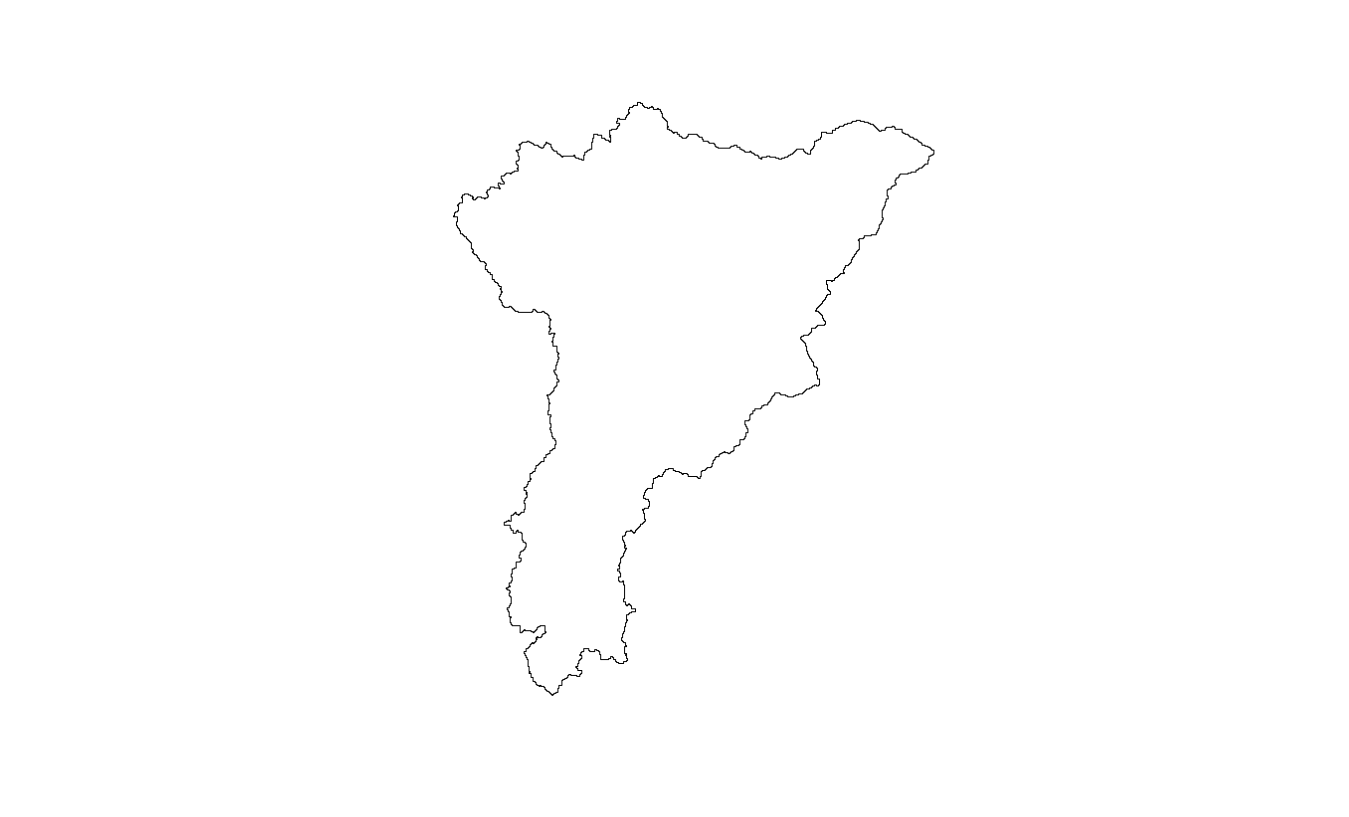
\includegraphics{form cu soc.png}
\caption{Forma de la Cuenca del Soco\label{mapauno}}
\end{figure}

\begin{figure}
\centering
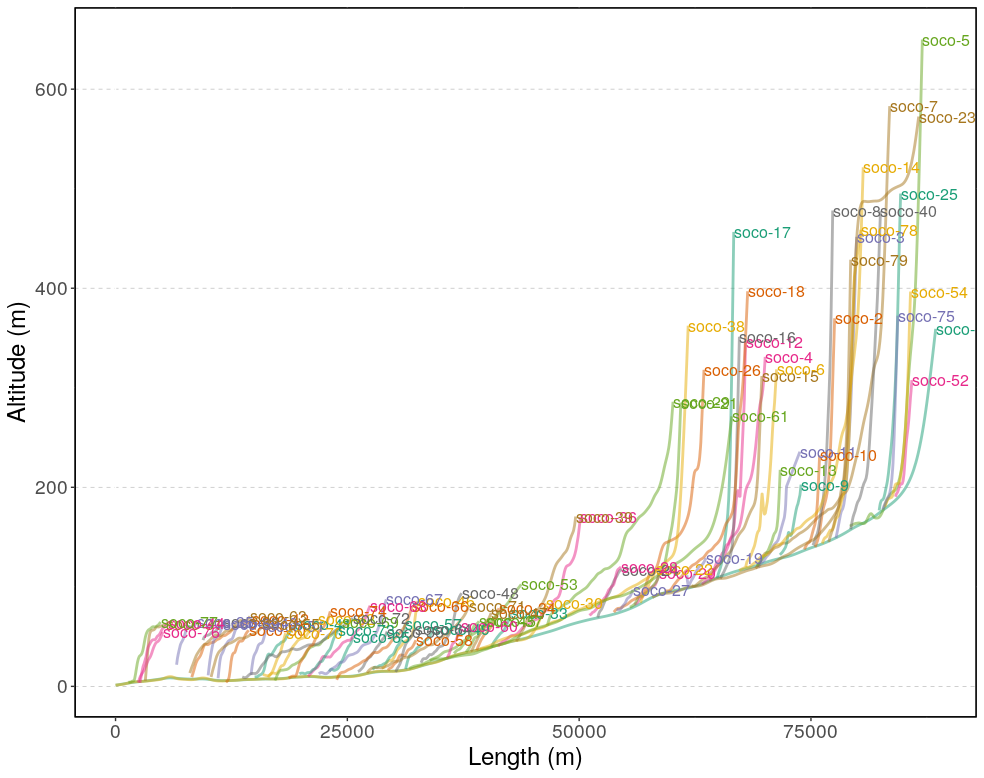
\includegraphics[width=0.50000\textwidth]{perf mas largo.png}
\caption{Perfiles Longitudinales de los cursos mas largos en la Cuenca
del Soco\label{mapauno}}
\end{figure}

\begin{figure}
\centering
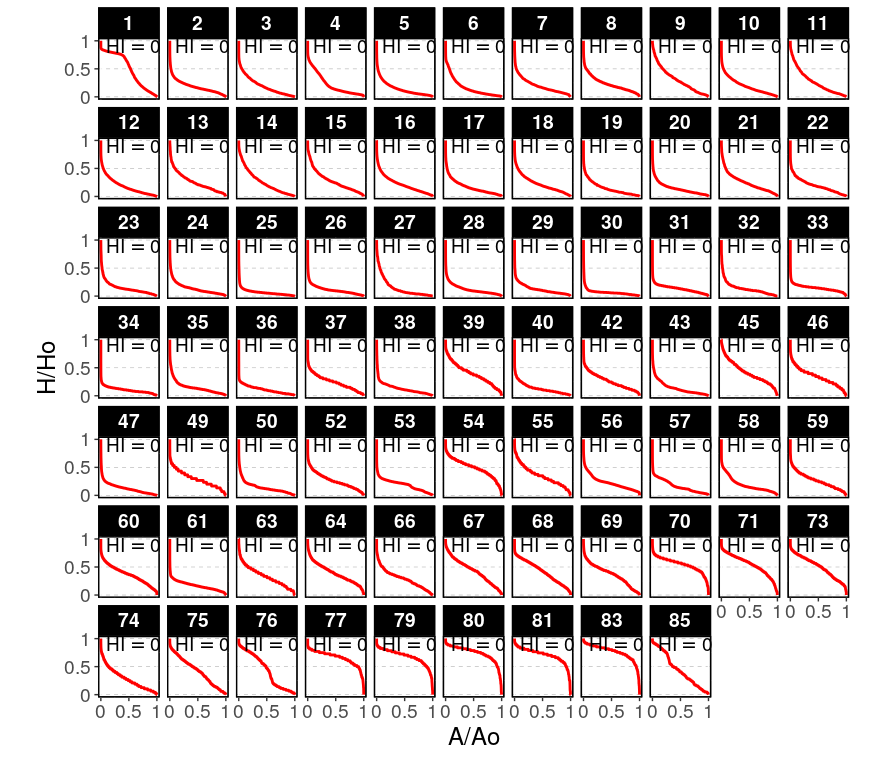
\includegraphics[width=0.70000\textwidth]{c de red o dos.png}
\caption{Cuenca de Orden de Red Numero 2\label{mapados}}
\end{figure}

\begin{figure}
\centering
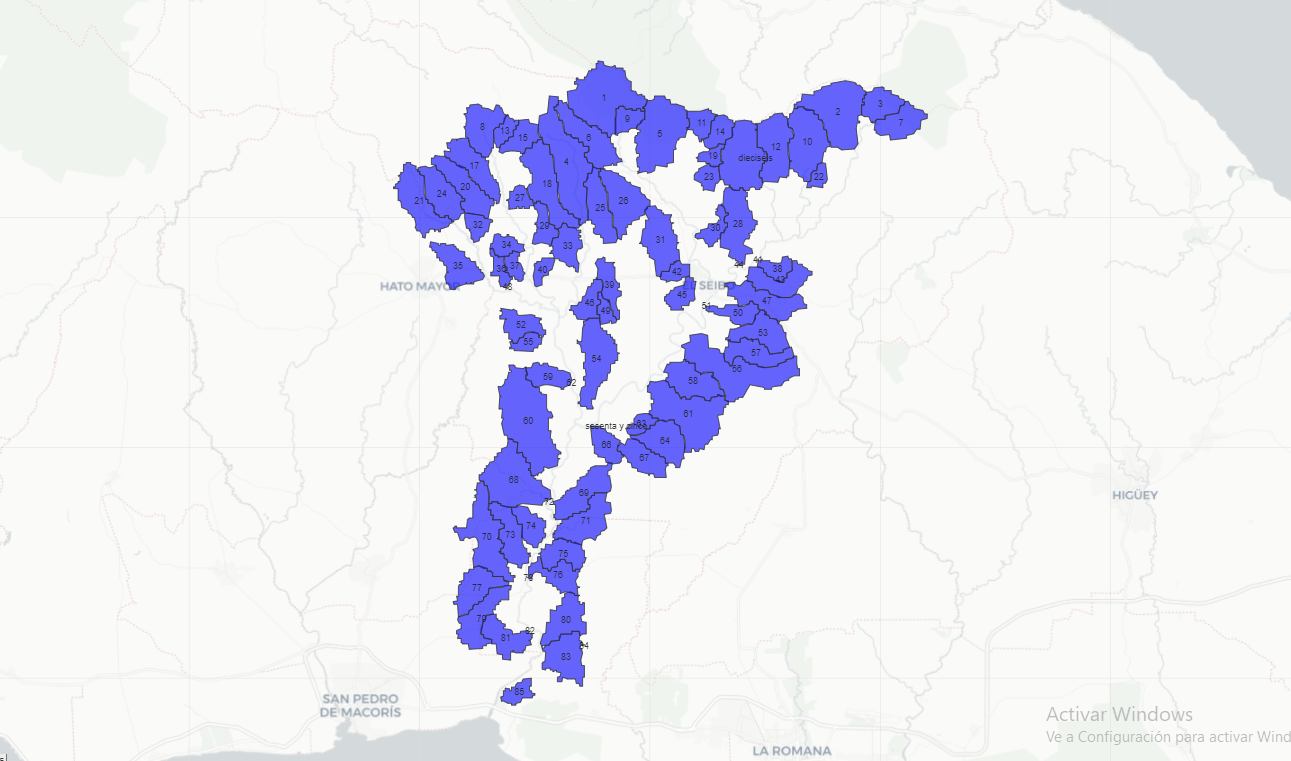
\includegraphics[width=0.70000\textwidth]{cu drena or dos.png}
\caption{Red de Drenaje de orden Dos\label{mapatres}}
\end{figure}

\begin{figure}
\centering
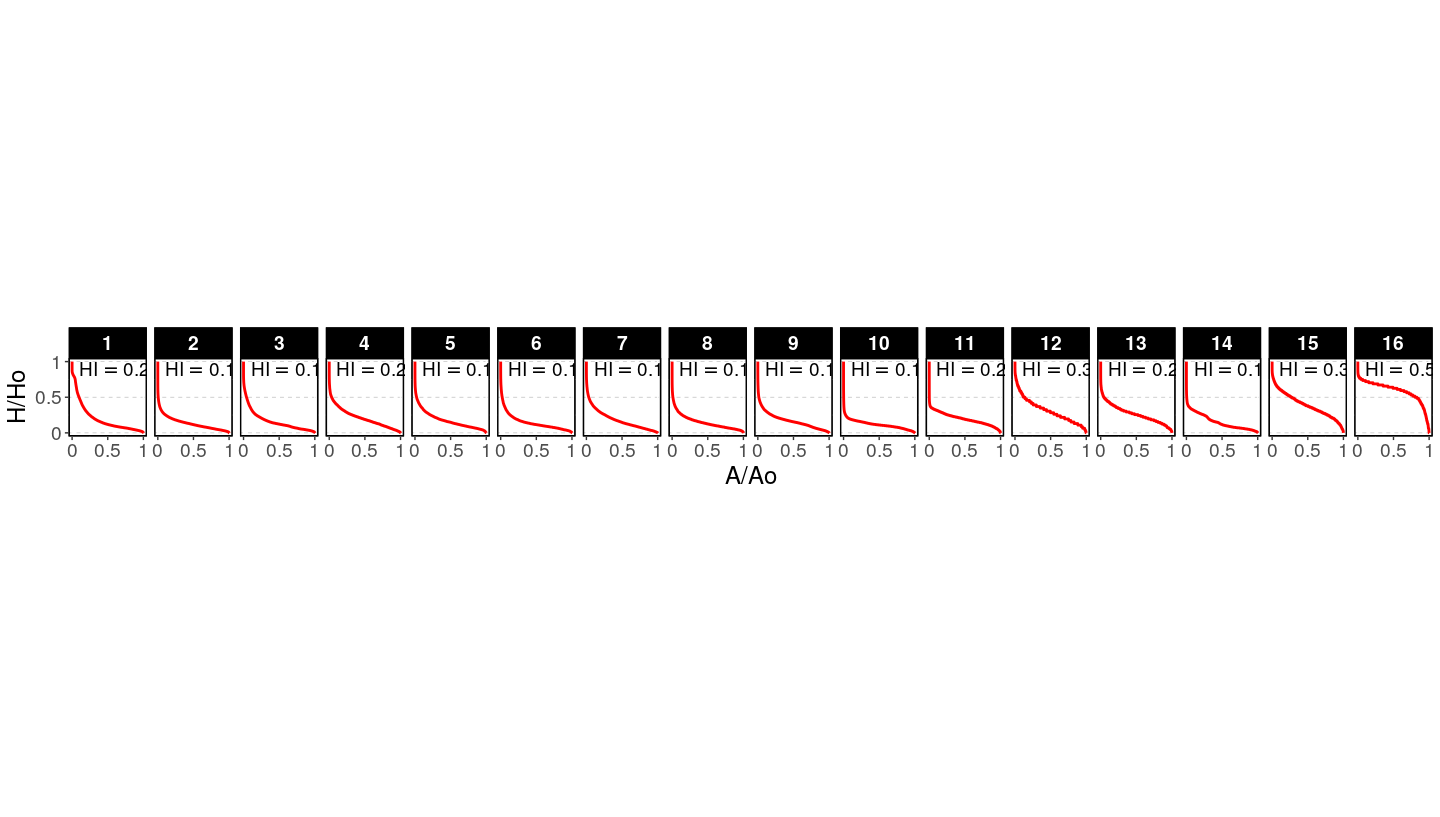
\includegraphics[width=0.70000\textwidth]{cu de red or tres.png}
\caption{Cuenca de Orden de Red Numero Tres\label{mapacuatro}}
\end{figure}

\begin{figure}
\centering
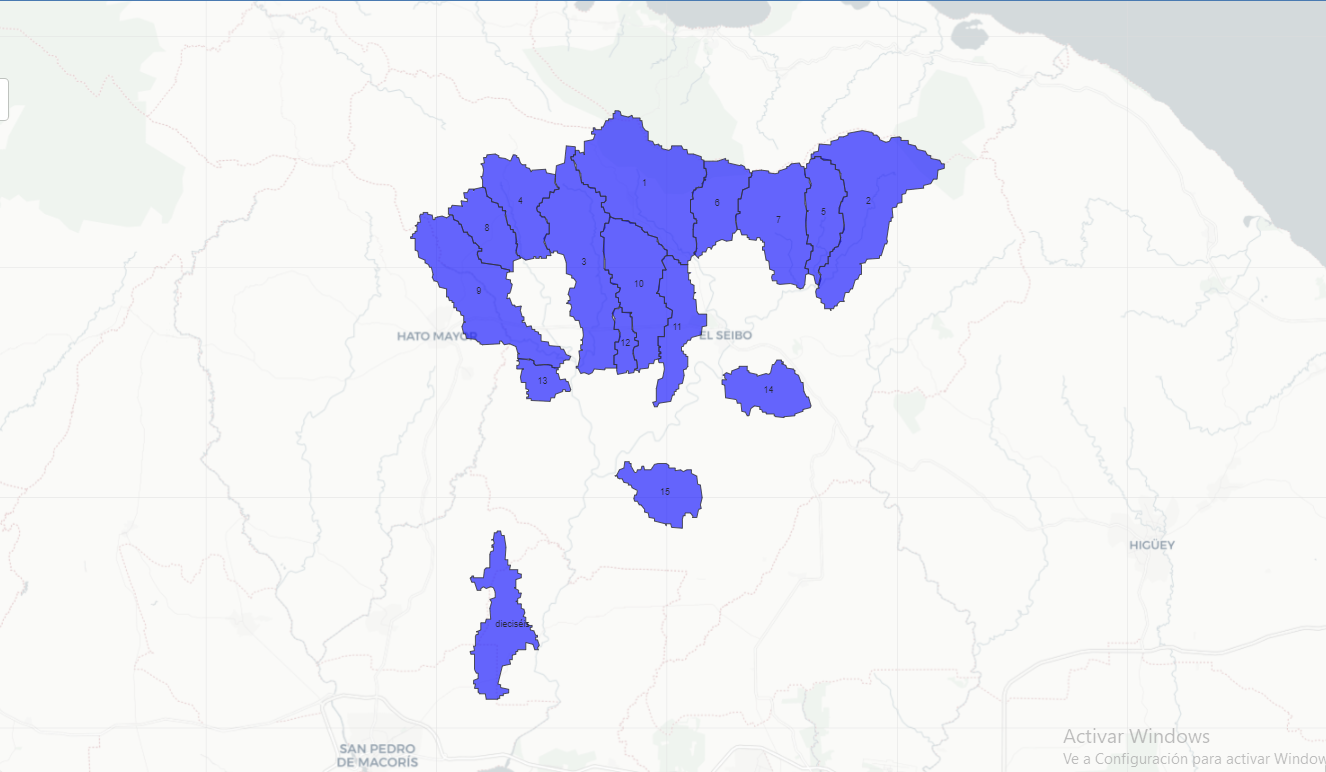
\includegraphics[width=0.70000\textwidth]{cu drena or tres.png}
\caption{Red de Drenaje de orden Dos\label{mapacinco}}
\end{figure}

\begin{figure}
\centering
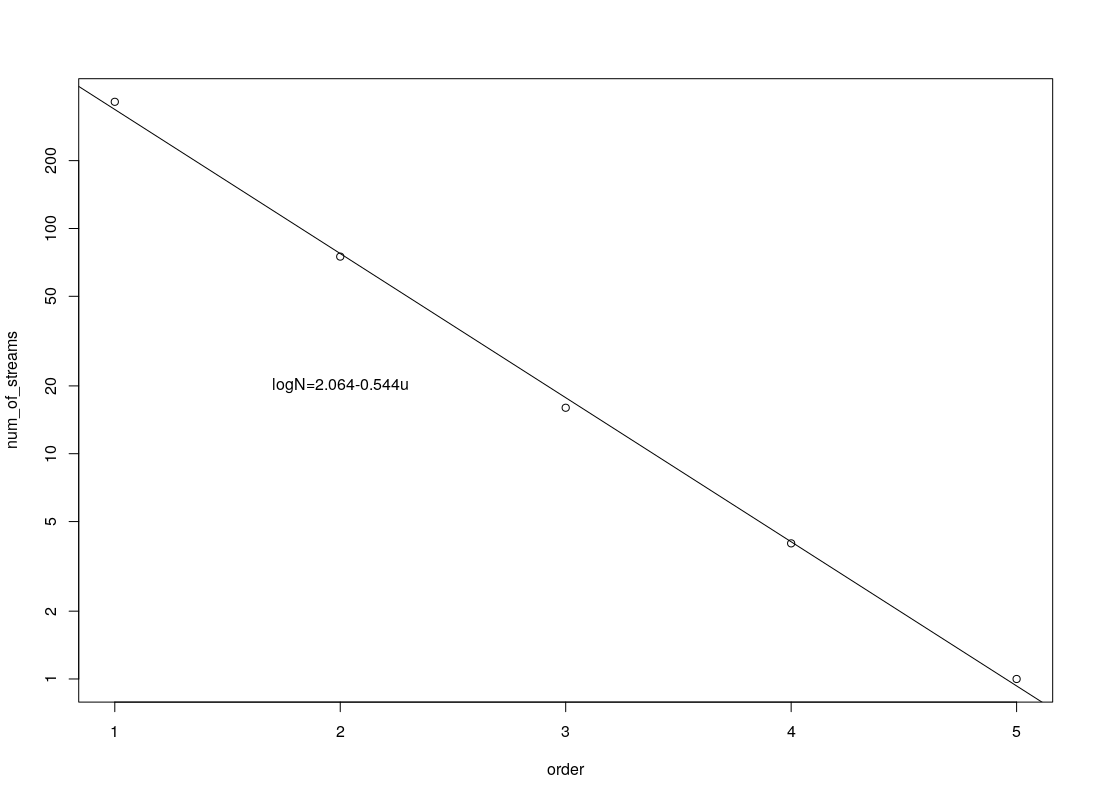
\includegraphics[width=0.70000\textwidth]{num redes razon bif.png}
\caption{Numero de ordenes de Redes y Razon de
Bifurcación\label{mapaseis}}
\end{figure}

\begin{figure}
\centering
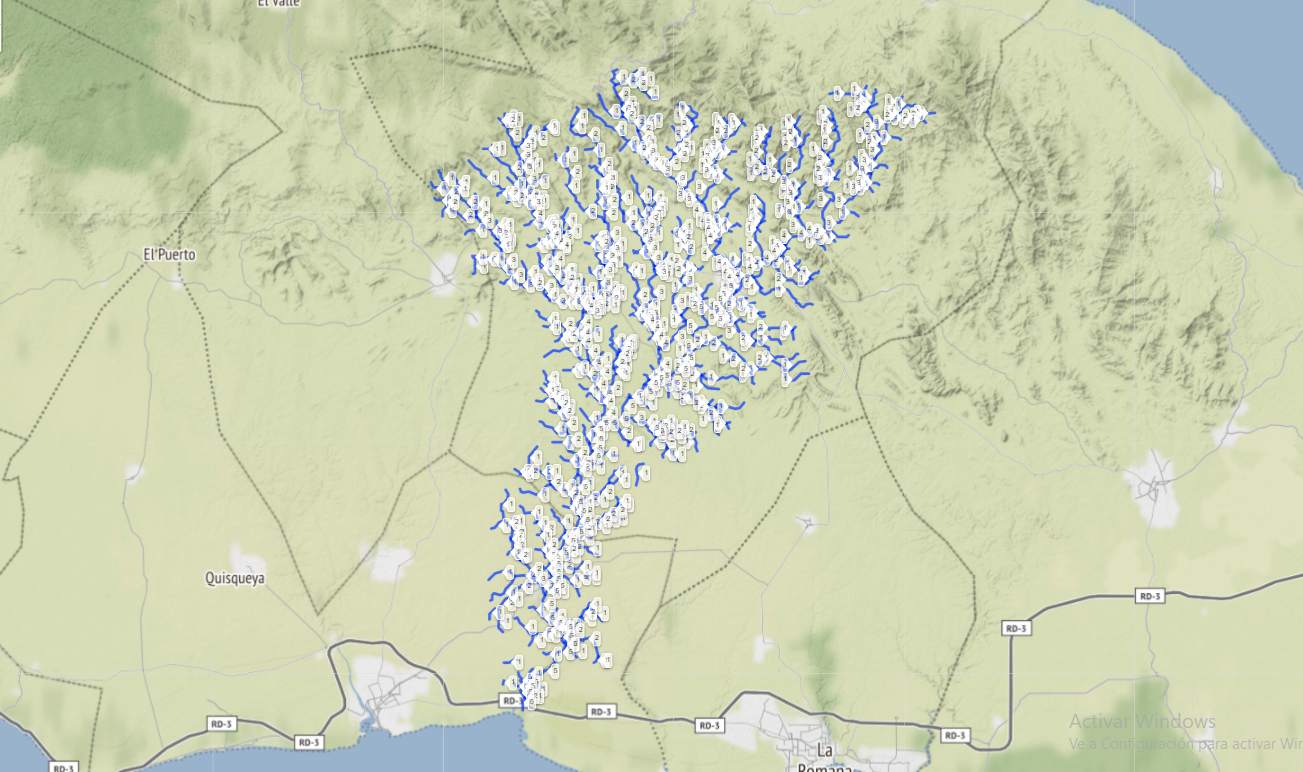
\includegraphics[width=0.70000\textwidth]{unica sim.png}
\caption{Ordenes de Red de la ceuenca del Soco con única
Simbología\label{mapasiete}}
\end{figure}

\begin{figure}
\centering
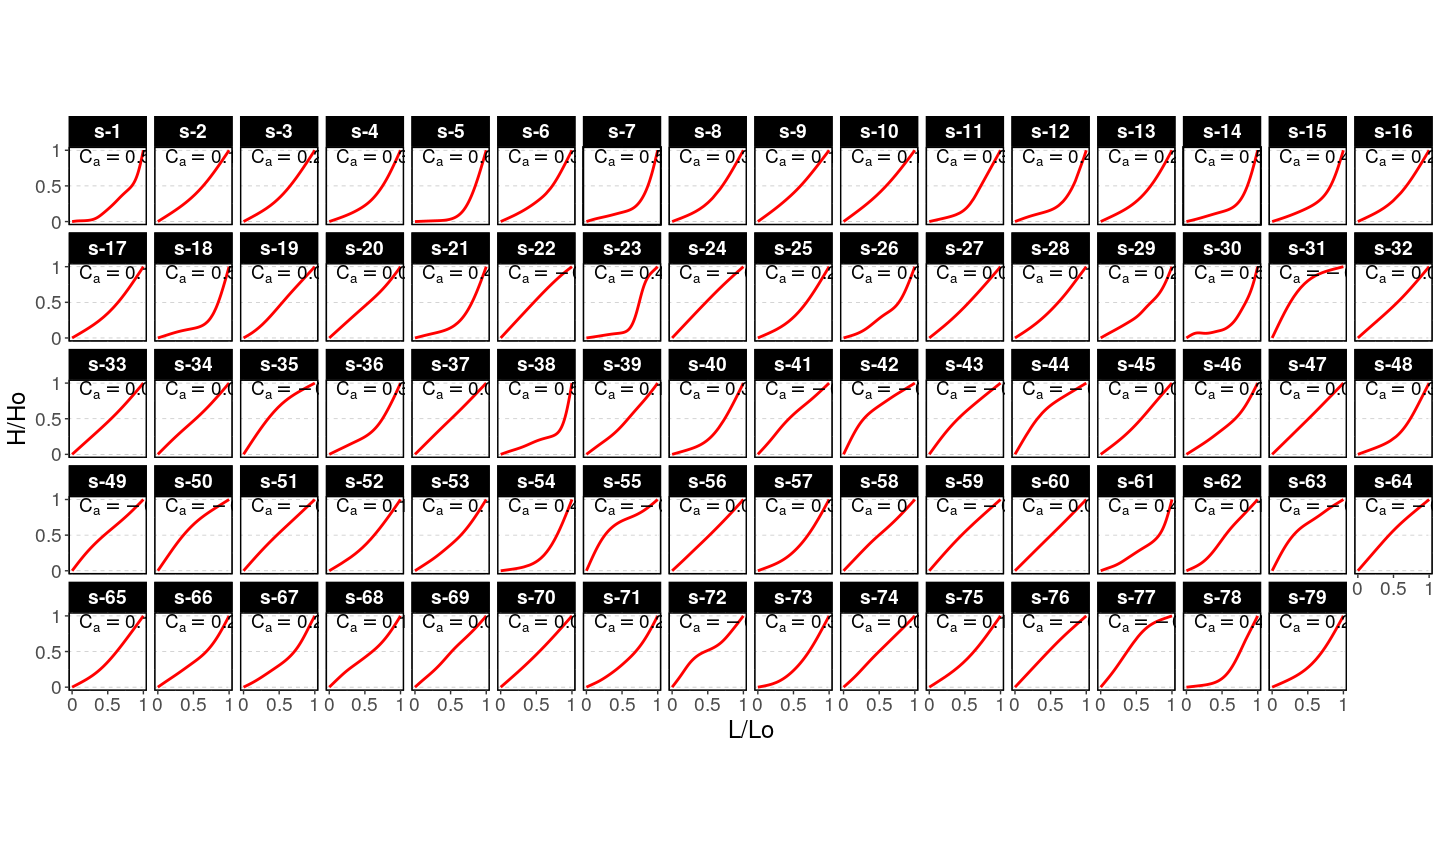
\includegraphics[width=0.70000\textwidth]{mas largos.png}
\caption{Perfiles Longitudinlaes e indices de concavidad de los cursos
mas largos de la cuenca del Soco\label{mapaocho}}
\end{figure}

\begin{figure}
\centering
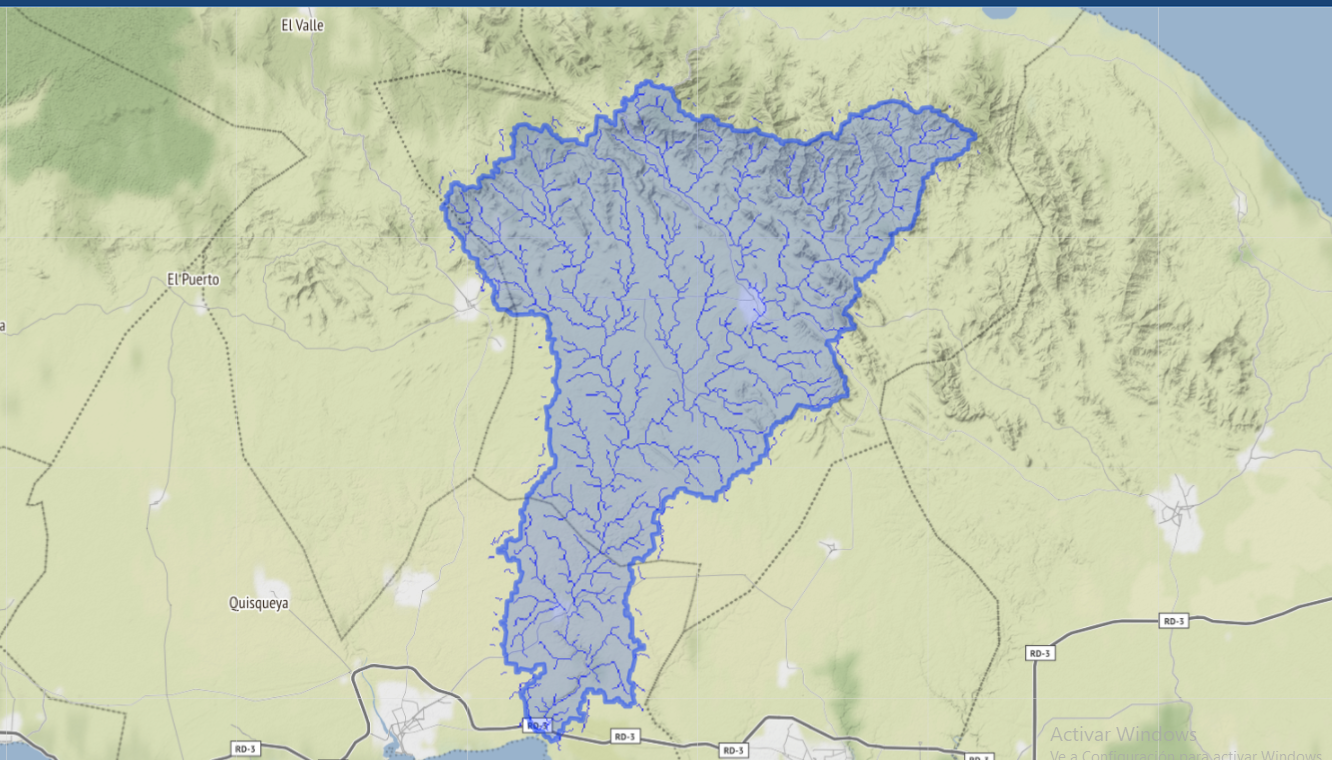
\includegraphics[width=0.70000\textwidth]{denaje.png}
\caption{Red de Drenaje de la Cuenca del Soco\label{mapanueve}}
\end{figure}

\begin{figure}
\centering
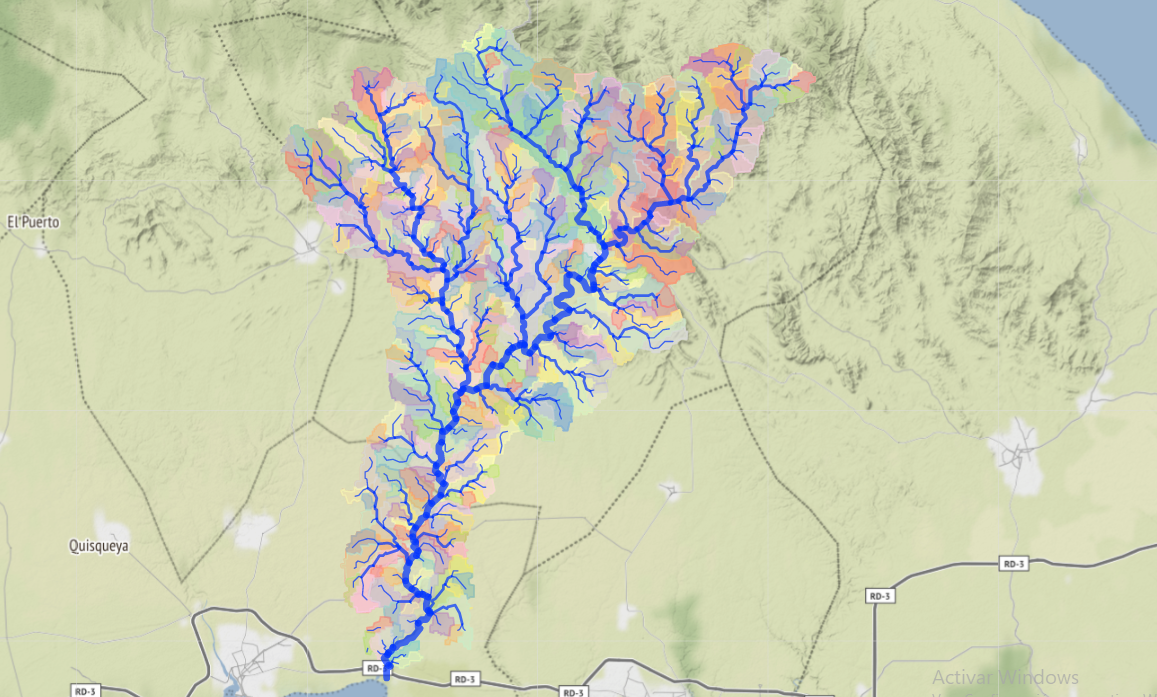
\includegraphics[width=0.70000\textwidth]{drenaje segun orden.png}
\caption{Red de Drenaje según su Orden de Red en la Cuenca del
Soco\label{mapadiez}}
\end{figure}

\begin{longtable}[]{@{}llllll@{}}
\caption{\label{tablacuatro}Variables promediadas para cada orden de
red.}\tabularnewline
\toprule
\begin{minipage}[b]{0.12\columnwidth}\raggedright\strut
Order Num\strut
\end{minipage} & \begin{minipage}[b]{0.13\columnwidth}\raggedright\strut
Avg.len (km)\strut
\end{minipage} & \begin{minipage}[b]{0.13\columnwidth}\raggedright\strut
Avg.ar (km2)\strut
\end{minipage} & \begin{minipage}[b]{0.13\columnwidth}\raggedright\strut
Avg.sl (m/m)\strut
\end{minipage} & \begin{minipage}[b]{0.16\columnwidth}\raggedright\strut
Avg.grad. (m/m)\strut
\end{minipage} & \begin{minipage}[b]{0.15\columnwidth}\raggedright\strut
Avg.el.dif (m)\strut
\end{minipage}\tabularnewline
\midrule
\endfirsthead
\toprule
\begin{minipage}[b]{0.12\columnwidth}\raggedright\strut
Order Num\strut
\end{minipage} & \begin{minipage}[b]{0.13\columnwidth}\raggedright\strut
Avg.len (km)\strut
\end{minipage} & \begin{minipage}[b]{0.13\columnwidth}\raggedright\strut
Avg.ar (km2)\strut
\end{minipage} & \begin{minipage}[b]{0.13\columnwidth}\raggedright\strut
Avg.sl (m/m)\strut
\end{minipage} & \begin{minipage}[b]{0.16\columnwidth}\raggedright\strut
Avg.grad. (m/m)\strut
\end{minipage} & \begin{minipage}[b]{0.15\columnwidth}\raggedright\strut
Avg.el.dif (m)\strut
\end{minipage}\tabularnewline
\midrule
\endhead
\begin{minipage}[t]{0.12\columnwidth}\raggedright\strut
1\strut
\end{minipage} & \begin{minipage}[t]{0.13\columnwidth}\raggedright\strut
1.0951\strut
\end{minipage} & \begin{minipage}[t]{0.13\columnwidth}\raggedright\strut
1.6194\strut
\end{minipage} & \begin{minipage}[t]{0.13\columnwidth}\raggedright\strut
0.0218\strut
\end{minipage} & \begin{minipage}[t]{0.16\columnwidth}\raggedright\strut
0.0162\strut
\end{minipage} & \begin{minipage}[t]{0.15\columnwidth}\raggedright\strut
17.6603\strut
\end{minipage}\tabularnewline
\begin{minipage}[t]{0.12\columnwidth}\raggedright\strut
2\strut
\end{minipage} & \begin{minipage}[t]{0.13\columnwidth}\raggedright\strut
2.9720\strut
\end{minipage} & \begin{minipage}[t]{0.13\columnwidth}\raggedright\strut
8.3544\strut
\end{minipage} & \begin{minipage}[t]{0.13\columnwidth}\raggedright\strut
0.0133\strut
\end{minipage} & \begin{minipage}[t]{0.16\columnwidth}\raggedright\strut
0.0100\strut
\end{minipage} & \begin{minipage}[t]{0.15\columnwidth}\raggedright\strut
33.2667\strut
\end{minipage}\tabularnewline
\begin{minipage}[t]{0.12\columnwidth}\raggedright\strut
3\strut
\end{minipage} & \begin{minipage}[t]{0.13\columnwidth}\raggedright\strut
6.0900\strut
\end{minipage} & \begin{minipage}[t]{0.13\columnwidth}\raggedright\strut
34.1317\strut
\end{minipage} & \begin{minipage}[t]{0.13\columnwidth}\raggedright\strut
0.0081\strut
\end{minipage} & \begin{minipage}[t]{0.16\columnwidth}\raggedright\strut
0.0049\strut
\end{minipage} & \begin{minipage}[t]{0.15\columnwidth}\raggedright\strut
31.2500\strut
\end{minipage}\tabularnewline
\begin{minipage}[t]{0.12\columnwidth}\raggedright\strut
4\strut
\end{minipage} & \begin{minipage}[t]{0.13\columnwidth}\raggedright\strut
12.4215\strut
\end{minipage} & \begin{minipage}[t]{0.13\columnwidth}\raggedright\strut
157.2015\strut
\end{minipage} & \begin{minipage}[t]{0.13\columnwidth}\raggedright\strut
0.0063\strut
\end{minipage} & \begin{minipage}[t]{0.16\columnwidth}\raggedright\strut
0.0030\strut
\end{minipage} & \begin{minipage}[t]{0.15\columnwidth}\raggedright\strut
38.2500\strut
\end{minipage}\tabularnewline
\begin{minipage}[t]{0.12\columnwidth}\raggedright\strut
5\strut
\end{minipage} & \begin{minipage}[t]{0.13\columnwidth}\raggedright\strut
57.8980\strut
\end{minipage} & \begin{minipage}[t]{0.13\columnwidth}\raggedright\strut
983.8981\strut
\end{minipage} & \begin{minipage}[t]{0.13\columnwidth}\raggedright\strut
0.0076\strut
\end{minipage} & \begin{minipage}[t]{0.16\columnwidth}\raggedright\strut
0.0015\strut
\end{minipage} & \begin{minipage}[t]{0.15\columnwidth}\raggedright\strut
87.0000\strut
\end{minipage}\tabularnewline
\bottomrule
\end{longtable}

\begin{longtable}[]{@{}llllll@{}}
\caption{\label{tablacinco}Desviacion estandar para las estadisticas
segfun orden de red}\tabularnewline
\toprule
\begin{minipage}[b]{0.13\columnwidth}\raggedright\strut
Order Num\strut
\end{minipage} & \begin{minipage}[b]{0.13\columnwidth}\raggedright\strut
Std.len (km)\strut
\end{minipage} & \begin{minipage}[b]{0.13\columnwidth}\raggedright\strut
Std.ar (km2)\strut
\end{minipage} & \begin{minipage}[b]{0.13\columnwidth}\raggedright\strut
Std.sl (m/m)\strut
\end{minipage} & \begin{minipage}[b]{0.15\columnwidth}\raggedright\strut
Std.grad (m/m)\strut
\end{minipage} & \begin{minipage}[b]{0.15\columnwidth}\raggedright\strut
Std.el.dif (m)\strut
\end{minipage}\tabularnewline
\midrule
\endfirsthead
\toprule
\begin{minipage}[b]{0.13\columnwidth}\raggedright\strut
Order Num\strut
\end{minipage} & \begin{minipage}[b]{0.13\columnwidth}\raggedright\strut
Std.len (km)\strut
\end{minipage} & \begin{minipage}[b]{0.13\columnwidth}\raggedright\strut
Std.ar (km2)\strut
\end{minipage} & \begin{minipage}[b]{0.13\columnwidth}\raggedright\strut
Std.sl (m/m)\strut
\end{minipage} & \begin{minipage}[b]{0.15\columnwidth}\raggedright\strut
Std.grad (m/m)\strut
\end{minipage} & \begin{minipage}[b]{0.15\columnwidth}\raggedright\strut
Std.el.dif (m)\strut
\end{minipage}\tabularnewline
\midrule
\endhead
\begin{minipage}[t]{0.13\columnwidth}\raggedright\strut
1\strut
\end{minipage} & \begin{minipage}[t]{0.13\columnwidth}\raggedright\strut
0.8702\strut
\end{minipage} & \begin{minipage}[t]{0.13\columnwidth}\raggedright\strut
1.0490\strut
\end{minipage} & \begin{minipage}[t]{0.13\columnwidth}\raggedright\strut
0.0234\strut
\end{minipage} & \begin{minipage}[t]{0.15\columnwidth}\raggedright\strut
0.0174\strut
\end{minipage} & \begin{minipage}[t]{0.15\columnwidth}\raggedright\strut
21.0933\strut
\end{minipage}\tabularnewline
\begin{minipage}[t]{0.13\columnwidth}\raggedright\strut
2\strut
\end{minipage} & \begin{minipage}[t]{0.13\columnwidth}\raggedright\strut
2.3431\strut
\end{minipage} & \begin{minipage}[t]{0.13\columnwidth}\raggedright\strut
5.3580\strut
\end{minipage} & \begin{minipage}[t]{0.13\columnwidth}\raggedright\strut
0.0083\strut
\end{minipage} & \begin{minipage}[t]{0.15\columnwidth}\raggedright\strut
0.0076\strut
\end{minipage} & \begin{minipage}[t]{0.15\columnwidth}\raggedright\strut
47.5177\strut
\end{minipage}\tabularnewline
\begin{minipage}[t]{0.13\columnwidth}\raggedright\strut
3\strut
\end{minipage} & \begin{minipage}[t]{0.13\columnwidth}\raggedright\strut
4.2366\strut
\end{minipage} & \begin{minipage}[t]{0.13\columnwidth}\raggedright\strut
19.5514\strut
\end{minipage} & \begin{minipage}[t]{0.13\columnwidth}\raggedright\strut
0.0029\strut
\end{minipage} & \begin{minipage}[t]{0.15\columnwidth}\raggedright\strut
0.0023\strut
\end{minipage} & \begin{minipage}[t]{0.15\columnwidth}\raggedright\strut
20.9269\strut
\end{minipage}\tabularnewline
\begin{minipage}[t]{0.13\columnwidth}\raggedright\strut
4\strut
\end{minipage} & \begin{minipage}[t]{0.13\columnwidth}\raggedright\strut
7.8694\strut
\end{minipage} & \begin{minipage}[t]{0.13\columnwidth}\raggedright\strut
72.9224\strut
\end{minipage} & \begin{minipage}[t]{0.13\columnwidth}\raggedright\strut
0.0004\strut
\end{minipage} & \begin{minipage}[t]{0.15\columnwidth}\raggedright\strut
0.0005\strut
\end{minipage} & \begin{minipage}[t]{0.15\columnwidth}\raggedright\strut
8.2297\strut
\end{minipage}\tabularnewline
\begin{minipage}[t]{0.13\columnwidth}\raggedright\strut
5\strut
\end{minipage} & \begin{minipage}[t]{0.13\columnwidth}\raggedright\strut
0.0000\strut
\end{minipage} & \begin{minipage}[t]{0.13\columnwidth}\raggedright\strut
0.0000\strut
\end{minipage} & \begin{minipage}[t]{0.13\columnwidth}\raggedright\strut
0.0000\strut
\end{minipage} & \begin{minipage}[t]{0.15\columnwidth}\raggedright\strut
0.0000\strut
\end{minipage} & \begin{minipage}[t]{0.15\columnwidth}\raggedright\strut
0.0000\strut
\end{minipage}\tabularnewline
\bottomrule
\end{longtable}

\begin{longtable}[]{@{}llll@{}}
\caption{\label{tablaseis}Razones de los parametros hidrograficos segun
el orden de red}\tabularnewline
\toprule
Order & N.streams & Tot.len (km) & Tot.area (km2)\tabularnewline
\midrule
\endfirsthead
\toprule
Order & N.streams & Tot.len (km) & Tot.area (km2)\tabularnewline
\midrule
\endhead
1 & 365 & 399.7040 & 591.0968\tabularnewline
2 & 75 & 222.8964 & 626.5809\tabularnewline
3 & 16 & 97.4407 & 546.1068\tabularnewline
4 & 4 & 49.6858 & 628.8060\tabularnewline
5 & 1 & 57.8980 & 983.8981\tabularnewline
\bottomrule
\end{longtable}

\begin{longtable}[]{@{}llllllll@{}}
\caption{\label{tablasiete}Razones de los parametros hidrograficos segun
su orden de red}\tabularnewline
\toprule
Order & Bif.rt. & Len.rt. & Area.rt. & Slo.rt. & Grd.rt. & d.dens. &
str.freq.\tabularnewline
\midrule
\endfirsthead
\toprule
Order & Bif.rt. & Len.rt. & Area.rt. & Slo.rt. & Grd.rt. & d.dens. &
str.freq.\tabularnewline
\midrule
\endhead
1 & 4.8667 & 2.7139 & 0.0000 & 1.6406 & 1.6100 & 0.6762 &
0.6175\tabularnewline
2 & 4.6875 & 2.0492 & 5.1588 & 1.6358 & 2.0326 & 0.3557 &
0.1197\tabularnewline
3 & 4.0000 & 2.0396 & 4.0855 & 1.2922 & 1.6364 & 0.1784 &
0.0293\tabularnewline
4 & 4.0000 & 4.6611 & 4.6057 & 0.8313 & 2.0090 & 0.0790 &
0.0064\tabularnewline
5 & 0.0000 & 0.0000 & 6.2588 & 0.0000 & 0.0000 & 0.0588 &
0.0010\tabularnewline
\bottomrule
\end{longtable}

\begin{longtable}[]{@{}ll@{}}
\caption{\label{tablasiete}Parametros morfometricos de la Cuenca del
Soco}\tabularnewline
\toprule
\begin{minipage}[b]{0.66\columnwidth}\raggedright\strut
Parametros\strut
\end{minipage} & \begin{minipage}[b]{0.28\columnwidth}\raggedright\strut
Valores\strut
\end{minipage}\tabularnewline
\midrule
\endfirsthead
\toprule
\begin{minipage}[b]{0.66\columnwidth}\raggedright\strut
Parametros\strut
\end{minipage} & \begin{minipage}[b]{0.28\columnwidth}\raggedright\strut
Valores\strut
\end{minipage}\tabularnewline
\midrule
\endhead
\begin{minipage}[t]{0.66\columnwidth}\raggedright\strut
Easting Centroid of basin\strut
\end{minipage} & \begin{minipage}[t]{0.28\columnwidth}\raggedright\strut
489195.00\strut
\end{minipage}\tabularnewline
\begin{minipage}[t]{0.66\columnwidth}\raggedright\strut
Northing Centroid of basin\strut
\end{minipage} & \begin{minipage}[t]{0.28\columnwidth}\raggedright\strut
2072655.00\strut
\end{minipage}\tabularnewline
\begin{minipage}[t]{0.66\columnwidth}\raggedright\strut
Rectangle containing basin N-W\strut
\end{minipage} & \begin{minipage}[t]{0.28\columnwidth}\raggedright\strut
(`471060', `2092680')``\strut
\end{minipage}\tabularnewline
\begin{minipage}[t]{0.66\columnwidth}\raggedright\strut
Rectangle containing basin S-E\strut
\end{minipage} & \begin{minipage}[t]{0.28\columnwidth}\raggedright\strut
``(`513630', `2039760')''\strut
\end{minipage}\tabularnewline
\begin{minipage}[t]{0.66\columnwidth}\raggedright\strut
Area of basin {[}km2{]}\strut
\end{minipage} & \begin{minipage}[t]{0.28\columnwidth}\raggedright\strut
989.801775\strut
\end{minipage}\tabularnewline
\begin{minipage}[t]{0.66\columnwidth}\raggedright\strut
Perimeter of basin {[}km{]}\strut
\end{minipage} & \begin{minipage}[t]{0.28\columnwidth}\raggedright\strut
227.636525830754\strut
\end{minipage}\tabularnewline
\begin{minipage}[t]{0.66\columnwidth}\raggedright\strut
Max Elevation {[}m s.l.m.{]}\strut
\end{minipage} & \begin{minipage}[t]{0.28\columnwidth}\raggedright\strut
646.969411439852\strut
\end{minipage}\tabularnewline
\begin{minipage}[t]{0.66\columnwidth}\raggedright\strut
Min Elevation {[}m s.l.m.{]}\strut
\end{minipage} & \begin{minipage}[t]{0.28\columnwidth}\raggedright\strut
0.0326075545062636\strut
\end{minipage}\tabularnewline
\begin{minipage}[t]{0.66\columnwidth}\raggedright\strut
Elevation Difference {[}m{]}\strut
\end{minipage} & \begin{minipage}[t]{0.28\columnwidth}\raggedright\strut
646.9368038853457\strut
\end{minipage}\tabularnewline
\begin{minipage}[t]{0.66\columnwidth}\raggedright\strut
Mean Elevation\strut
\end{minipage} & \begin{minipage}[t]{0.28\columnwidth}\raggedright\strut
136.3463\strut
\end{minipage}\tabularnewline
\begin{minipage}[t]{0.66\columnwidth}\raggedright\strut
Mean Slope\strut
\end{minipage} & \begin{minipage}[t]{0.28\columnwidth}\raggedright\strut
4.65\strut
\end{minipage}\tabularnewline
\begin{minipage}[t]{0.66\columnwidth}\raggedright\strut
Length of Directing Vector {[}km{]}\strut
\end{minipage} & \begin{minipage}[t]{0.28\columnwidth}\raggedright\strut
33.6112628742212\strut
\end{minipage}\tabularnewline
\begin{minipage}[t]{0.66\columnwidth}\raggedright\strut
Prevalent Orientation {[}degree from north, counterclockwise{]}\strut
\end{minipage} & \begin{minipage}[t]{0.28\columnwidth}\raggedright\strut
1.250701649253028\strut
\end{minipage}\tabularnewline
\begin{minipage}[t]{0.66\columnwidth}\raggedright\strut
Compactness Coefficient\strut
\end{minipage} & \begin{minipage}[t]{0.28\columnwidth}\raggedright\strut
6.412284389087794\strut
\end{minipage}\tabularnewline
\begin{minipage}[t]{0.66\columnwidth}\raggedright\strut
Circularity Ratio\strut
\end{minipage} & \begin{minipage}[t]{0.28\columnwidth}\raggedright\strut
0.2400347916120\strut
\end{minipage}\tabularnewline
\begin{minipage}[t]{0.66\columnwidth}\raggedright\strut
Topological Diameter\strut
\end{minipage} & \begin{minipage}[t]{0.28\columnwidth}\raggedright\strut
,120.0\strut
\end{minipage}\tabularnewline
\begin{minipage}[t]{0.66\columnwidth}\raggedright\strut
Elongation Ratio\strut
\end{minipage} & \begin{minipage}[t]{0.28\columnwidth}\raggedright\strut
0.4103977285869175\strut
\end{minipage}\tabularnewline
\begin{minipage}[t]{0.66\columnwidth}\raggedright\strut
Shape Factor\strut
\end{minipage} & \begin{minipage}[t]{0.28\columnwidth}\raggedright\strut
,11.44258120713636\strut
\end{minipage}\tabularnewline
\begin{minipage}[t]{0.66\columnwidth}\raggedright\strut
``Concentration Time (Giandotti, 1934) {[}hr{]}\strut
\end{minipage} & \begin{minipage}[t]{0.28\columnwidth}\raggedright\strut
12.561301584730437\strut
\end{minipage}\tabularnewline
\begin{minipage}[t]{0.66\columnwidth}\raggedright\strut
Length of Mainchannel {[}km{]}\strut
\end{minipage} & \begin{minipage}[t]{0.28\columnwidth}\raggedright\strut
86.501616819\strut
\end{minipage}\tabularnewline
\begin{minipage}[t]{0.66\columnwidth}\raggedright\strut
Mean slope of mainchannel {[}percent{]}\strut
\end{minipage} & \begin{minipage}[t]{0.28\columnwidth}\raggedright\strut
1.0508578295624251\strut
\end{minipage}\tabularnewline
\begin{minipage}[t]{0.66\columnwidth}\raggedright\strut
Mean hillslope length {[}m{]}\strut
\end{minipage} & \begin{minipage}[t]{0.28\columnwidth}\raggedright\strut
311.9917\strut
\end{minipage}\tabularnewline
\begin{minipage}[t]{0.66\columnwidth}\raggedright\strut
Elevation Difference {[}m{]}\strut
\end{minipage} & \begin{minipage}[t]{0.28\columnwidth}\raggedright\strut
646.9368038853457\strut
\end{minipage}\tabularnewline
\begin{minipage}[t]{0.66\columnwidth}\raggedright\strut
Magnitudo,\strut
\end{minipage} & \begin{minipage}[t]{0.28\columnwidth}\raggedright\strut
289.0\strut
\end{minipage}\tabularnewline
\begin{minipage}[t]{0.66\columnwidth}\raggedright\strut
Max order (Strahler)\strut
\end{minipage} & \begin{minipage}[t]{0.28\columnwidth}\raggedright\strut
5\strut
\end{minipage}\tabularnewline
\begin{minipage}[t]{0.66\columnwidth}\raggedright\strut
Number of streams\strut
\end{minipage} & \begin{minipage}[t]{0.28\columnwidth}\raggedright\strut
421\strut
\end{minipage}\tabularnewline
\begin{minipage}[t]{0.66\columnwidth}\raggedright\strut
Total Stream Length {[}km{]}\strut
\end{minipage} & \begin{minipage}[t]{0.28\columnwidth}\raggedright\strut
815.5888\strut
\end{minipage}\tabularnewline
\begin{minipage}[t]{0.66\columnwidth}\raggedright\strut
First order stream frequency\strut
\end{minipage} & \begin{minipage}[t]{0.28\columnwidth}\raggedright\strut
0.2919776538085113\strut
\end{minipage}\tabularnewline
\begin{minipage}[t]{0.66\columnwidth}\raggedright\strut
Drainage Density {[}km/km\^{}2{]}\strut
\end{minipage} & \begin{minipage}[t]{0.28\columnwidth}\raggedright\strut
0.8239920563892704\strut
\end{minipage}\tabularnewline
\begin{minipage}[t]{0.66\columnwidth}\raggedright\strut
Bifurcation Ratio (Horton)\strut
\end{minipage} & \begin{minipage}[t]{0.28\columnwidth}\raggedright\strut
4.2453\strut
\end{minipage}\tabularnewline
\begin{minipage}[t]{0.66\columnwidth}\raggedright\strut
Length Ratio (Horton)\strut
\end{minipage} & \begin{minipage}[t]{0.28\columnwidth}\raggedright\strut
2.4703\strut
\end{minipage}\tabularnewline
\begin{minipage}[t]{0.66\columnwidth}\raggedright\strut
Area ratio (Horton)\strut
\end{minipage} & \begin{minipage}[t]{0.28\columnwidth}\raggedright\strut
4.6963\strut
\end{minipage}\tabularnewline
\begin{minipage}[t]{0.66\columnwidth}\raggedright\strut
Slope ratio (Horton)\strut
\end{minipage} & \begin{minipage}[t]{0.28\columnwidth}\raggedright\strut
1.3574\strut
\end{minipage}\tabularnewline
\bottomrule
\end{longtable}

\begin{longtable}[]{@{}lll@{}}
\caption{\label{tablaocho}Integral Hipsometrica en las cuencas de Orden
2}\tabularnewline
\toprule
ord & cat & Int. Hipso\tabularnewline
\midrule
\endfirsthead
\toprule
ord & cat & Int. Hipso\tabularnewline
\midrule
\endhead
1 & 1 & 0.48838926\tabularnewline
2 & 2 & 0.18193323\tabularnewline
3 & 3 & 0.19445524\tabularnewline
4 & 4 & 0.21762542\tabularnewline
5 & 5 & 0.14295602\tabularnewline
6 & 6 & 0.15991775\tabularnewline
7 & 7 & 0.19598821\tabularnewline
8 & 8 & 0.22972788\tabularnewline
9 & 9 & 0.29999456\tabularnewline
10 & 10 & 0.19312651\tabularnewline
11 & 11 & 0.26362902\tabularnewline
12 & 12 & 0.18092041\tabularnewline
13 & 13 & 0.25637129\tabularnewline
14 & 14 & 0.25578278\tabularnewline
15 & 15 & 0.27399930\tabularnewline
16 & 16 & 0.21718352\tabularnewline
17 & 17 & 0.16731969\tabularnewline
18 & 18 & 0.22313861\tabularnewline
19 & 19 & 0.14558501\tabularnewline
20 & 20 & 0.14253386\tabularnewline
21 & 21 & 0.24687863\tabularnewline
22 & 22 & 0.19453870\tabularnewline
23 & 23 & 0.14312417\tabularnewline
24 & 24 & 0.13588177\tabularnewline
25 & 25 & 0.06656511\tabularnewline
26 & 26 & 0.10905142\tabularnewline
27 & 27 & 0.14094699\tabularnewline
28 & 28 & 0.11947547\tabularnewline
29 & 29 & 0.12154615\tabularnewline
30 & 30 & 0.06694574\tabularnewline
31 & 31 & 0.12986863\tabularnewline
32 & 32 & 0.13214347\tabularnewline
33 & 33 & 0.14299769\tabularnewline
34 & 34 & 0.10321406\tabularnewline
35 & 35 & 0.14836356\tabularnewline
36 & 36 & 0.10991497\tabularnewline
37 & 37 & 0.24081809\tabularnewline
38 & 38 & 0.12914719\tabularnewline
39 & 39 & 0.38783102\tabularnewline
40 & 40 & 0.13000859\tabularnewline
41 & 42 & 0.25771843\tabularnewline
42 & 43 & 0.13739951\tabularnewline
43 & 45 & 0.41175533\tabularnewline
44 & 46 & 0.33664967\tabularnewline
45 & 47 & 0.12660206\tabularnewline
46 & 49 & 0.29142210\tabularnewline
47 & 50 & 0.14173861\tabularnewline
48 & 52 & 0.26207370\tabularnewline
49 & 53 & 0.18704006\tabularnewline
50 & 54 & 0.48698763\tabularnewline
51 & 55 & 0.34952735\tabularnewline
52 & 56 & 0.22693968\tabularnewline
53 & 57 & 0.16492509\tabularnewline
54 & 58 & 0.18884589\tabularnewline
55 & 59 & 0.26409218\tabularnewline
56 & 60 & 0.36586150\tabularnewline
57 & 61 & 0.16777662\tabularnewline
58 & 63 & 0.33413105\tabularnewline
59 & 64 & 0.38969687\tabularnewline
60 & 66 & 0.28774555\tabularnewline
61 & 67 & 0.43177657\tabularnewline
62 & 68 & 0.41594979\tabularnewline
63 & 69 & 0.36691619\tabularnewline
64 & 70 & 0.54537122\tabularnewline
65 & 71 & 0.54050406\tabularnewline
66 & 73 & 0.50115083\tabularnewline
67 & 74 & 0.28375791\tabularnewline
68 & 75 & 0.41880781\tabularnewline
69 & 76 & 0.43451360\tabularnewline
70 & 77 & 0.65887177\tabularnewline
71 & 79 & 0.68029357\tabularnewline
72 & 80 & 0.73798593\tabularnewline
73 & 81 & 0.70710689\tabularnewline
74 & 83 & 0.76043899\tabularnewline
75 & 85 & 0.44416178\tabularnewline
\bottomrule
\end{longtable}

\begin{longtable}[]{@{}lll@{}}
\caption{\label{tablanueve}Integral Hipsometrica en las cuencas de orden
3}\tabularnewline
\toprule
ord & cat & Int. Hipso\tabularnewline
\midrule
\endfirsthead
\toprule
ord & cat & Int. Hipso\tabularnewline
\midrule
\endhead
1 & 1 & 0.1969233\tabularnewline
2 & 2 & 0.1351459\tabularnewline
3 & 3 & 0.1620187\tabularnewline
4 & 4 & 0.2090313\tabularnewline
5 & 5 & 0.1767976\tabularnewline
6 & 6 & 0.1462086\tabularnewline
7 & 7 & 0.1822861\tabularnewline
8 & 8 & 0.1504306\tabularnewline
9 & 9 & 0.1708137\tabularnewline
10 & 10 & 0.1184473\tabularnewline
11 & 11 & 0.1967438\tabularnewline
12 & 12 & 0.3106096\tabularnewline
13 & 13 & 0.2661533\tabularnewline
14 & 14 & 0.1557006\tabularnewline
15 & 15 & 0.3884555\tabularnewline
16 & 16 & 0.5907859\tabularnewline
\bottomrule
\end{longtable}

\ldots

\section{\texorpdfstring{\emph{Script}
reproducible}{Script reproducible}}\label{script-reproducible}

\ldots

\section*{Referencias}\label{referencias}
\addcontentsline{toc}{section}{Referencias}

\hypertarget{refs}{}
\hypertarget{ref-busnelli2014morfometria}{}
Busnelli, J., \& Horta, L. R. (2014). Morfometría de cuencas montañas y
metamorfosis fluvial, tucumán. \emph{Revista de La Asociación Geológica
Argentina}, \emph{71}(1), 11--20.

\hypertarget{ref-allaire2012rstudio}{}
Citeseer (Ed.). (n.d.). RStudio: Entorno de desarrollo integrado para r.
\emph{Boston, MA}.

\hypertarget{ref-warmerdam2005gdal}{}
GDAL-biblioteca de abstracción de datos geoespaciales. (n.d.).
\emph{Http: // Www. Gdal. Org /}.

\hypertarget{ref-jain2003adding}{}
Jain, T., Siddharth y Barclay. (n.d.). \emph{Adición de epsg: 4326
geographic longitude-latitude projection a terraserver} (agosto, Ed.).

\hypertarget{ref-jasiewicz2011new}{}
Jasiewicz, M., Jaros ~l aw y Metz. (n.d.). Un nuevo juego de
herramientas grass gis para el análisis hortoniano de redes de drenaje.
\emph{Computers ~\& Geosciences}.

\hypertarget{ref-lemos2004avaliaccao}{}
Lemos, M., Souza, S., \& Rocha, R. (2004). Avaliação da qualidade dos
dados altimétricos derivado do shuttle radar topographic mission (srtm):
Resultados preliminares. \emph{Anais I Simpósio Em Ciências Geodésicas E
Tecnologias Da Geoinformação, Recife}, 1--3.

\hypertarget{ref-lozar2003geographic}{}
Lozar, C. R. y C., Robert C y Ehlschlaeger. (n.d.). \emph{Un enfoque de
sistemas de información geográfica (sig) e imágenes para las tendencias
históricas de crecimiento urbano en torno a las instalaciones
militares}.

\hypertarget{ref-moussa2009definition}{}
Moussa, R. (2009). Definition of new equivalent indices of
horton-strahler ratios for the derivation of the geomorphological
instantaneous unit hydrograph. \emph{Water Resources Research},
\emph{45}(9).

\hypertarget{ref-munoz2009geomorfologia}{}
Muñoz-Rojas, J., Carrasco González, R. M., \& Pedraza Gilsanz, J. de.
(2009). Geomorfología regional y ordenación integral del territorio:
Nuevas perspectivas basadas en la incertidumbre y la complejidad de las
formas del terreno. aplicación en la cuenca del río bullaque (montes de
toledo, españa). \emph{Boletín de La Real Sociedad Española de Historia
Natural. Sección Geológica}, \emph{103}(1-4), 23--47.

\hypertarget{ref-ollero2011innovacion}{}
Ollero, A., Ibisate, A., Acín, V., Díaz, E., Granado, D., \& Horacio, J.
(2011). Innovación y libertad fluvial. \emph{Comunicación vii congreso
ibérico sobre gestión y planificación del agua}.

\hypertarget{ref-di2013open}{}
Un enfoque de código abierto para la caracterización fisiográfica de la
cuenca. (n.d.). \emph{Resúmenes de la reunión de otoño de agu}.




\newpage
\singlespacing 
\end{document}
